\subsection{Opret Projekt}
Dette afsnit indeholder en gennemgang af grafisk brugergrænseflade, design og implementering af Opret Projekt viewet i Rambøll Tilsyn.

\subsubsection{Design}
På figur \ref{fig:OpretProjektSekvens} ses sekvens diagrammet for opret bruger viewet til Rambøll Tilsyn.
\begin{figure}[H] % (alternativt [H])
	\centering
	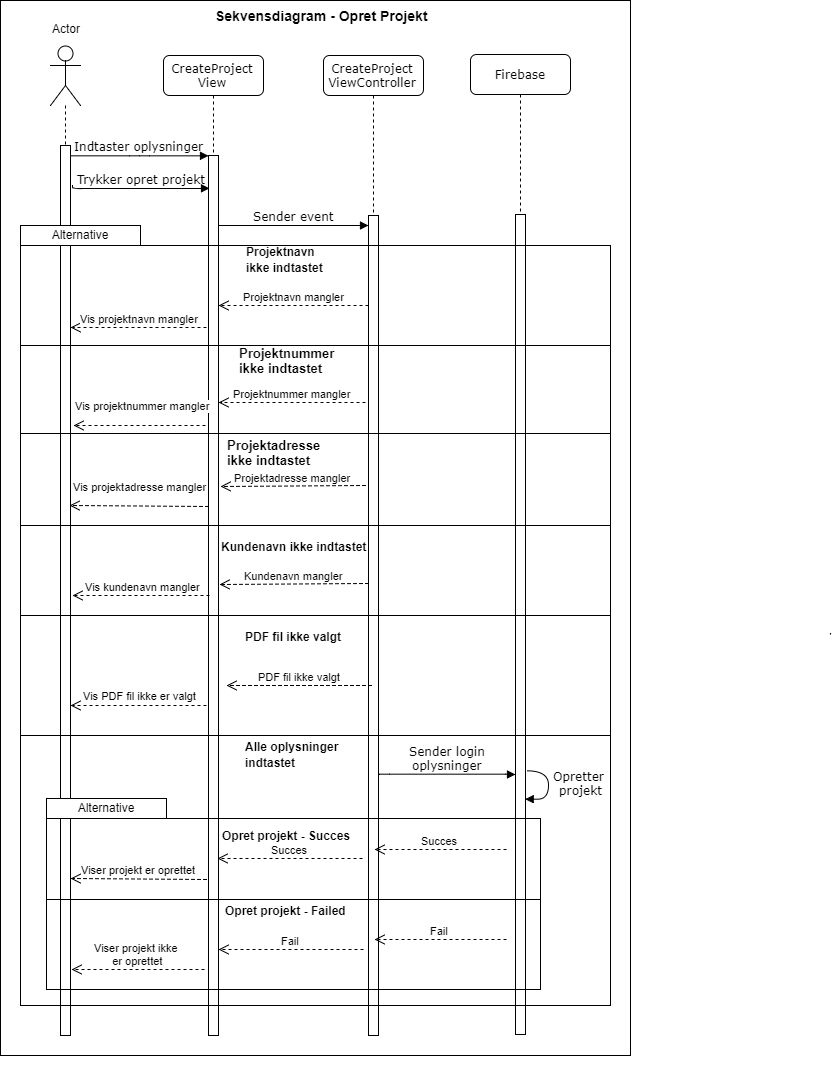
\includegraphics[height=20cm, width=15cm]{../ArkitekturDesign/Design/OpretProjekt/OpretProjektSekvensDiagram}
	\caption{Sekvensdiagram for Opret Bruger i Rambøll Tilsyn.}
	\label{fig:OpretProjektSekvens}
\end{figure}

\subsubsection{Grafisk brugergrænseflade}
I OpretProjektViewet er der lavet felter til alt det information, som skal tastes ind om et projekt. Se figur \ref{fig:OpretProjektView}
\begin{figure}[H] % (alternativt [H])
	\centering
	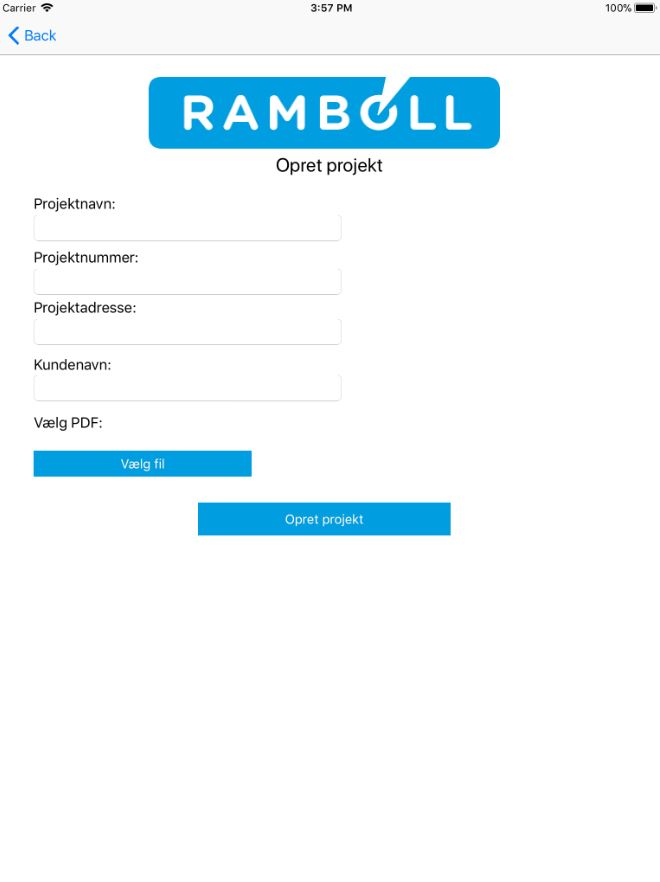
\includegraphics[height=12cm, width=10cm]{../ArkitekturDesign/Design/OpretProjekt/OpretProjektView}
	\caption{Opret projekt viewet som det er implementeret i Rambøll Tilsyn.}
	\label{fig:OpretProjektView}
\end{figure}

\subsubsection{Implementering}
Når der skal oprettes et nyt projekt, validerer controlleren at der er indtastet information i alle felter,
inden at informationen bliver sendt videre til modellen. Hvis et felt ikke er udfyldt giver controlleren fejlbesked til viewet. \\

\clearpage